\documentclass[a4paper]{article}
\usepackage{vntex}
%\usepackage[english,vietnam]{babel}
%\usepackage[utf8]{inputenc}

%\usepackage[utf8]{inputenc}
%\usepackage[francais]{babel}
\usepackage{a4wide,amssymb,epsfig,latexsym,multicol,array,hhline,fancyhdr}
\usepackage{booktabs}
\usepackage{amsmath}
\usepackage{lastpage}
\usepackage[lined,boxed,commentsnumbered]{algorithm2e}
\usepackage{enumerate}
\usepackage{color}
\usepackage{graphicx}							% Standard graphics package
\usepackage{array}
\usepackage{tabularx, caption}
\usepackage{multirow}
\usepackage[framemethod=tikz]{mdframed}% For highlighting paragraph backgrounds
\usepackage{multicol}
\usepackage{rotating}
\usepackage{graphics}
\usepackage{geometry}
\usepackage{setspace}
\usepackage{epsfig}
\usepackage{tikz}
\usepackage{float}
\usepackage{listings}
\usetikzlibrary{arrows,snakes,backgrounds}
\usepackage{hyperref}
\hypersetup{urlcolor=blue,linkcolor=black,citecolor=black,colorlinks=true} 
%\usepackage{pstcol} 								% PSTricks with the standard color package

\newtheorem{theorem}{{\bf Định lý}}
\newtheorem{property}{{\bf Tính chất}}
\newtheorem{proposition}{{\bf Mệnh đề}}
\newtheorem{corollary}[proposition]{{\bf Hệ quả}}
\newtheorem{lemma}[proposition]{{\bf Bổ đề}}

\everymath{\color{blue}}
%\usepackage{fancyhdr}
\setlength{\headheight}{40pt}
\pagestyle{fancy}
\fancyhead{} % clear all header fields
\fancyhead[L]{
 \begin{tabular}{rl}
    \begin{picture}(25,15)(0,0)
    \put(0,-8){
\includegraphics[width=8mm, height=8mm]{logoITSGUsmall.png}}
    %\put(0,-8){\epsfig{width=10mm,figure=hcmut.eps}}
   \end{picture}&
	%\includegraphics[width=8mm, height=8mm]{hcmut.png} & %
	\begin{tabular}{l}
		\textbf{\bf \ttfamily Trường Đại học Sài Gòn}\\
		\textbf{\bf \ttfamily Khoa Công Nghệ Thông Tin}
	\end{tabular} 	
 \end{tabular}
}
\fancyhead[R]{
	\begin{tabular}{l}
		\tiny \bf \\
		\tiny \bf 
	\end{tabular}  }
\fancyfoot{} % clear all footer fields
\fancyfoot[L]{\scriptsize \ttfamily Bài tập môn Công Nghệ Phần Mềm - Niên khóa 2024-2025}
\fancyfoot[R]{\scriptsize \ttfamily Trang {\thepage}/\pageref{LastPage}}
\renewcommand{\headrulewidth}{0.3pt}
\renewcommand{\footrulewidth}{0.3pt}


%%%
\setcounter{secnumdepth}{4}
\setcounter{tocdepth}{3}
\makeatletter
\newcounter {subsubsubsection}[subsubsection]
\renewcommand\thesubsubsubsection{\thesubsubsection .\@alph\c@subsubsubsection}
\newcommand\subsubsubsection{\@startsection{subsubsubsection}{4}{\z@}%
                                     {-3.25ex\@plus -1ex \@minus -.2ex}%
                                     {1.5ex \@plus .2ex}%
                                     {\normalfont\normalsize\bfseries}}
\newcommand*\l@subsubsubsection{\@dottedtocline{3}{10.0em}{4.1em}}
\newcommand*{\subsubsubsectionmark}[1]{}
\makeatother

\definecolor{dkgreen}{rgb}{0,0.6,0}
\definecolor{gray}{rgb}{0.5,0.5,0.5}
\definecolor{mauve}{rgb}{0.58,0,0.82}

\lstset{frame=tb,
	language=Matlab,
	aboveskip=3mm,
	belowskip=3mm,
	showstringspaces=false,
	columns=flexible,
	basicstyle={\small\ttfamily},
	numbers=none,
	numberstyle=\tiny\color{gray},
	keywordstyle=\color{blue},
	commentstyle=\color{dkgreen},
	stringstyle=\color{mauve},
	breaklines=true,
	breakatwhitespace=true,
	tabsize=3,
	numbers=left,
	stepnumber=1,
	numbersep=1pt,    
	firstnumber=1,
	numberfirstline=true
}

\begin{document}

\begin{titlepage}
\begin{center}
TRƯỜNG ĐẠI HỌC SÀI GÒN \\
KHOA CÔNG NGHỆ THÔNG TIN
\end{center}
\vspace{1cm}

\begin{figure}[h!]
\begin{center}

\includegraphics[width=3cm]{logoITSGU.png}
\end{center}
\end{figure}

\vspace{1cm}


\begin{center}
\begin{tabular}{c}
	\multicolumn{1}{l}{\textbf{{\Large Công nghệ phần mềm}}}\\
	~~\\
	\hline
	\\
	\multicolumn{1}{l}{\textbf{{\Large  }}}\\
	\\
	
	\textbf{{\Huge Ứng dụng Đặt hàng \& Nhà hàng}}\\
	\\
	\hline
\end{tabular}
\end{center}

\vspace{3cm}

\begin{table}[h]
\begin{tabular}{rrl}
\hspace{5 cm} & GVHD: &Từ Lãng Phiêu\\
\hspace{5 cm} & NHÓM: &2\\
& SV: & Nguyễn Thanh Hiền - 3123560024 \\
& & Nhan Chí Phong - 3123560062 \\
& & Hoàng Đình Phú Quý - 3123560074 \\
& & Nguyễn Việt Hoàng - 3122560022 \\
& & Nguyễn Thành An - 3122410003 \\

\end{tabular}
\vspace{1.5 cm}
\end{table}

\begin{center}

{\footnotesize TP. HỒ CHÍ MINH, THÁNG 2/2024}
\end{center}
\end{titlepage}


\thispagestyle{empty}

\newpage
\tableofcontents
\newpage

%%%%%%%%%%%%%%%%%%%%%%%%%%%%%%%%%


%%%%%%%%%%%%%%%%%%%%%%%%%%%%%%%%%
\section{Giới thiệu}
\subsection{Tổng quan về hệ thống quản lý nhà hàng}

Ứng dụng web quản lý nhà hàng là một hệ thống toàn diện được phát triển nhằm quản lý hiệu quả các hoạt động của nhà hàng, từ quản lý thực đơn, đặt bàn, xử lý đơn hàng đến quản lý nguyên liệu và kho hàng. Hệ thống được xây dựng với kiến trúc phân tách rõ ràng giữa front-end và back-end.

\subsection{Bối cảnh của dự án}
Hiện nay, các nhà hàng đang sử dụng máy POS truyền thống để quản lý giao dịch và hoạt động hàng ngày. Tuy nhiên, chủ doanh nghiệp mong muốn nâng cao hiệu quả kinh doanh bằng cách cải tiến hệ thống hiện tại, bổ sung các chức năng mới để tối ưu trải nghiệm khách hàng và quy trình vận hành.

\subsection{Các bên liên quan chính}
\begin{itemize}
    \item \textbf{Chủ nhà hàng}: Người đưa ra quyết định và yêu cầu hệ thống, mong muốn vận hành có quy trình chặt chẽ và có khả năng mở rộng trong tương lai.
    \item \textbf{Khách hàng}: Sử dụng hệ thống đặt món bằng cách quét QR dẫn đến một giao diện được triển khai web, không cần giao tiếp với nhân viên.
    \item \textbf{Nhân viên}: Quản lý đơn hàng, chuẩn bị món, kiểm tra và xác nhận thanh toán của khách.
    \item \textbf{Nhóm phát triển phần mềm}: Xây dựng và triển khai hệ thống theo yêu cầu.
\end{itemize}

\subsection{Kỳ vọng sẽ được thực hiện}
\begin{itemize}
    \item Khách hàng thao tác quét QR, được điều hướng đến một trang web (không cần khách hàng tốn công cài đặt phần mềm vào điện thoại) nơi đó khách hàng gửi yêu cầu đặt món, không cần trao đổi với nhân viên.
    \item Nhà hàng sẽ được mở rộng trong tương lai nên cần phần mềm tối ưu khả năng giao dịch và xử lý đơn hàng.
    \item Thay thế POS truyền thống bằng hệ thống thao tác trên web, hỗ trợ đặt hàng, thanh toán, quản lý đơn hàng.
    \item Tối ưu hóa quy trình đặt hàng và đảm bảo quy trình làm việc chuyên nghiệp, trong trường hợp này lỗi thiếu sót đặt nhầm món và hay quên từ nhân viên phục vụ sẽ được khắc phục, cũng như giảm thiểu thời gian ghi nhận lại đơn hàng của khách trong trường hợp họ đi đông người và gọi quá nhiều món. Phù hợp khi khách hàng đi đông người và cần đặt rất nhiều món.
\end{itemize}

\subsection{Phạm vi của dự án}
\begin{itemize}
    \item Xây dựng hệ thống thao tác đặt món, đặt bàn, thanh toán trên web từ mã QR.
    \item Tích hợp quản lý menu, thông báo đơn hàng đến bếp và thanh toán qua nhiều hình thức.
    \item Có tiềm năng mở rộng dự án.
    \item Thiết kế các giao diện dành riêng trên mobile và web cho từng đối tượng người dùng tương ứng.
\end{itemize}

\subsection{Yêu cầu chức năng}
\begin{itemize}
\item \textbf{Quản lý khách hàng:}
  \begin{itemize}
    \item Thêm xem sửa xóa thông tin khách hàng.
    \item Phân loại khách hàng truy cập. (Từ website, qua QR tại quán)
    \item Lưu trữ lịch sử mua hàng của khách hàng.
    \item Tạo chương trình khách hàng thân thiết.
  \end{itemize}

\item \textbf{Quản lý nguyên liệu:}
  \begin{itemize}
    \item Thêm sửa xóa tạo nguyên liệu.
    \item Quản lý nhập nguyên liệu.
  \end{itemize}

\item \textbf{Quản lý món:} 
  \begin{itemize}
    \item Thêm, sửa, xóa các món, món ăn kèm/gia vị.
    \item Quản lý danh mục món ăn.
    \item Tìm kiếm và lọc món theo nhiều tiêu chí.
  \end{itemize}

\item \textbf{Quản lý đơn hàng:}
  \begin{itemize}
    \item Tạo đơn hàng, sửa đơn hàng.
    \item Xem danh sách đơn hàng, theo dõi trạng thái đơn hàng.
    \item Xóa đơn hàng chưa xác nhận thanh toán.
  \end{itemize}

\item \textbf{Quản lý đặt bàn:}
  \begin{itemize}
    \item Tạo lịch đặt bàn, khung giờ đặt và chi nhánh tùy theo lựa chọn khách hàng.
    \item Kiểm tra số bàn trống, xem vị trí bàn.
    \item Xem menu tham khảo.
    \item Ràng buộc yêu cầu đặt bàn. (Đặt trước 1 ngày và trong tuần)
  \end{itemize}

\item \textbf{Quản lý thanh toán:}
  \begin{itemize}
    \item Hỗ trợ thanh toán trực tuyến (tài khoản ngân hàng, ví điện tử, tiền mặt).
    \item Tính toán tổng tiền và giảm giá.
    \item Xuất hóa đơn điện tử.
  \end{itemize}
 
\item \textbf{Quản lý người dùng:}
  \begin{itemize}
    \item Đăng ký, đăng nhập cho người dùng.
    \item Phân quyền cho các vai trò (quản trị viên, nhân viên, khách hàng).
  \end{itemize}

\item \textbf{Quản lý doanh thu:}
  \begin{itemize}
    \item Tạo báo cáo doanh thu theo ngày/tháng.
    \item Thống kê lượt đặt bàn, đặt món.
    \item Hệ thống phân tích xu hướng món ăn bán chạy.
  \end{itemize}
\end{itemize}

\subsection{Yêu cầu phi chức năng}
\begin{itemize}
\item \textbf{Hiệu năng:}
  \begin{itemize}
    \item Thời gian tải trang ≤ 3 giây.
    \item Xử lý tối đa 100 giao dịch đồng thời.
    \item Tốc độ phản hồi < 1 giây cho mỗi thao tác.
  \end{itemize}
  
\item \textbf{Bảo mật:}
  \begin{itemize}
    \item Mã hóa dữ liệu nhạy cảm (tài khoản, giao dịch).
    \item Xác thực hai yếu tố cho thanh toán.
    \item Quản lý quyền truy cập chặt chẽ.
  \end{itemize}
  
\item \textbf{Độ tin cậy:}
  \begin{itemize}
    \item Sao lưu dữ liệu tự động, đảm bảo không mất dữ liệu.
    \item Hoạt động ổn định trong khung giờ 8h–22h.
  \end{itemize}
  
\item \textbf{Yêu cầu về tổ chức phần mềm:}
  \begin{itemize}
    \item Phần mềm có khả năng mở rộng trong tương lai
    \item Giao diện thân thiện, dễ sử dụng cho cả khách hàng và nhân viên.
    \item Hệ thống cần dễ dàng bảo trì và cập nhật mà không làm gián đoạn dịch vụ.
  \end{itemize}
  
\item \textbf{Yêu cầu ngoại cảnh:}
  \begin{itemize}
    \item Đảm bảo bảo mật thông tin khách hàng, nhân viên, quản lý.
    \item Tuân thủ quy định về thanh toán điện tử và bảo vệ dữ liệu cá nhân.
  \end{itemize}
\end{itemize}

\section{Kiến trúc hệ thống}
    \subsection{Tổng quan kiến trúc}
    
    Dự án được phát triển với kiến trúc microservices, phân tách rõ ràng giữa frontend và backend, giúp dễ dàng mở rộng và bảo trì.
    
    \subsubsection{Frontend (Next.js)}
    \begin{itemize}
        \item Giao diện khách hàng và nhân viên
        \item Tối ưu hóa hiệu suất với server-side rendering và static generation
        \item Quản lý trạng thái với Context API
        \item Giao diện người dùng hiện đại và responsive
    \end{itemize}
    
    \subsubsection{Backend (NestJS)}
    \begin{itemize}
        \item API RESTful xử lý logic nghiệp vụ
        \item Kiến trúc module rõ ràng với dependency injection
        \item Xác thực và phân quyền với JWT
        \item Tích hợp MongoDB qua Mongoose
        \item Xử lý email và thông báo
    \end{itemize}
    
    \subsection{Mô hình dữ liệu}
    
    Hệ thống sử dụng các schema sau để quản lý dữ liệu:
    
    \begin{enumerate}
        \item \textbf{Account}: Quản lý tài khoản người dùng
        \item \textbf{Customer}: Quản lý thông tin khách hàng
        \item \textbf{Table}: Quản lý bàn ăn và mã QR
        \item \textbf{Order}: Quản lý đơn hàng
        \item \textbf{OrderDetail}: Chi tiết đơn hàng
        \item \textbf{Dish}: Thông tin món ăn
        \item \textbf{Option}: Các tùy chọn cho món ăn
        \item \textbf{OptionGroup}: Nhóm tùy chọn
        \item \textbf{Recipe}: Công thức chế biến
        \item \textbf{Ingredient}: Nguyên liệu
        \item \textbf{Inventory}: Quản lý kho hàng
    \end{enumerate}

\newpage
\section{Phát triển dự án}
    \subsection{Các sơ đồ của hệ thống}
    \begin{itemize}
        \subsubsection{Task 1.3 - Use case}
        \begin{figure}[H]
            \centering
            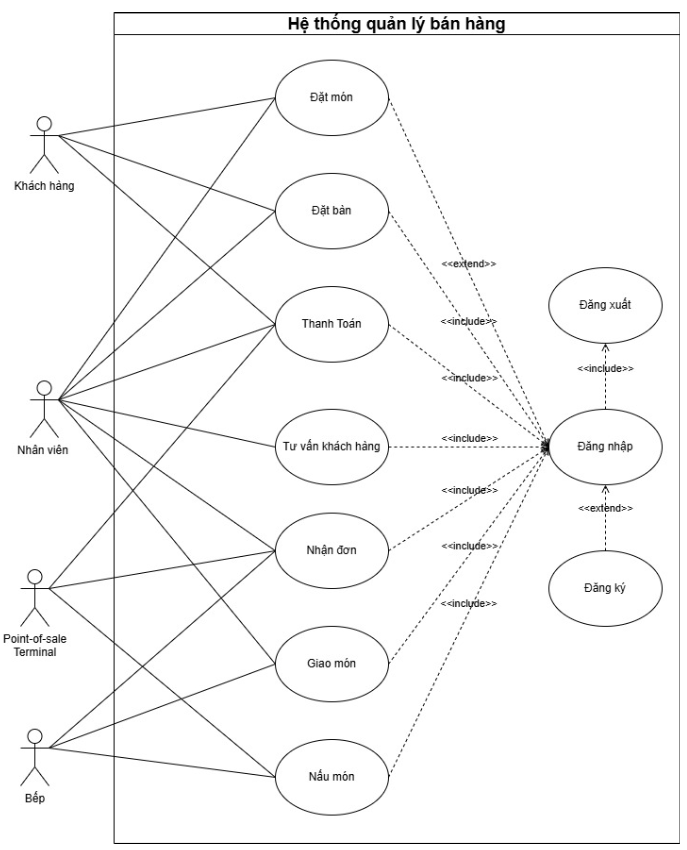
\includegraphics[width=0.8\textwidth]{task13.png}
            \caption{Sơ đồ Use Case của hệ thống}
            \label{fig:task13}
        \end{figure}
        \item Đặc tả use case:
        
        \begin{table}[H]
            \centering
            \begin{tabular}{|p{3cm}|p{12cm}|}
                \hline
                \textbf{Tên use case} & Đặt bàn \\
                \hline
                \textbf{Tóm tắt} & Khách hàng truy cập website, đăng nhập (hoặc đăng ký nếu chưa có tài khoản) và thực hiện thao tác đặt bàn theo chính sách (đặt trước 1 ngày, chỉ trong tuần). Hệ thống ghi nhận yêu cầu đặt bàn và gửi thông báo cho hệ thống đặt bàn. Hệ thống đặt bàn sau đó kiểm tra thông tin đặt bàn, xác nhận và cập nhật trạng thái đặt bàn trên hệ thống. \\
                \hline
                \textbf{Tác nhân} & Khách hàng, hệ thống đặt bàn \\
                \hline
                \textbf{Tiền điều kiện} & 
                \begin{itemize}
                    \item Khách hàng đã có tài khoản
                    \item Đặt bàn: đặt trước 1 ngày, chỉ cho ngày trong tuần.
                \end{itemize} \\
                \hline
                \textbf{Hậu điều kiện} & 
                \begin{itemize}
                    \item Yêu cầu đặt bàn đã được ghi nhận và xử lý thành công trên hệ thống.
                    \item Hệ thống đặt bàn có danh sách các đặt bàn đã được xác nhận để chuẩn bị phục vụ khách hàng vào ngày đã đặt.
                \end{itemize} \\
                \hline
                \textbf{Luồng chính} & 
                1. Khách hàng:
                \begin{itemize}
                    \item Truy cập website qua link có sẵn.
                    \item Đăng nhập hoặc đăng ký tài khoản với thông tin cần thiết.
                    \item Chọn chức năng "Đặt bàn".
                    \item Nhập thông tin đặt bàn: ngày, giờ, số lượng khách, chi nhánh.
                    \item Xác nhận thông tin và gửi yêu cầu đặt bàn.
                \end{itemize}
                
                2. Hệ thống:
                \begin{itemize}
                    \item Kiểm tra tính hợp lệ của thông tin đặt bàn (đủ thông tin, tuân thủ chính sách đặt trước 1 ngày và trong tuần).
                    \item Ghi nhận yêu cầu và chuyển thông tin đặt bàn tới nhân viên quản lý.
                \end{itemize}
                
                3. Hệ thống đặt bàn:
                \begin{itemize}
                    \item Nhận thông báo về yêu cầu đặt bàn từ hệ thống.
                    \item Kiểm tra thông tin đặt bàn, xác minh lịch trình và khả năng phục vụ của quán.
                    \item Xác nhận yêu cầu đặt bàn (hoặc liên hệ khách hàng nếu cần điều chỉnh/chốt lại chi tiết).
                    \item Cập nhật trạng thái đặt bàn trên hệ thống và gửi xác nhận cuối cùng tới khách hàng.
                \end{itemize} \\
                \hline
                \textbf{Luồng thay thế} & 
                1. Lỗi đăng nhập/đăng ký: Nếu khách hàng nhập sai thông tin hoặc gặp lỗi trong quá trình đăng nhập, hệ thống sẽ thông báo lỗi và yêu cầu nhập lại thông tin.
                
                2. Yêu cầu đặt bàn không hợp lệ: Nếu khách hàng cố gắng đặt bàn vào ngày không thuộc chính sách (ví dụ: hôm nay hoặc cuối tuần), hệ thống sẽ hiển thị thông báo lỗi và hướng dẫn khách hàng chọn ngày hợp lệ.
                
                3. Thông tin đặt bàn cần xác nhận thêm: Nếu hệ thống đặt bàn phát hiện có yêu cầu đặc biệt (ví dụ: số lượng khách quá đông so với sức chứa quán hoặc yêu cầu đặt chỗ riêng biệt), nó sẽ không chấp nhận yêu cầu và gửi cảnh báo để điều chỉnh thông tin trước khi xác nhận. \\
                \hline
            \end{tabular}
            \label{tab:usecase-table}
        \end{table}
        \subsubsection{Task 2.1 - Sơ đồ hoạt động (Activity diagram)}
        \begin{figure}[H]
            \centering
            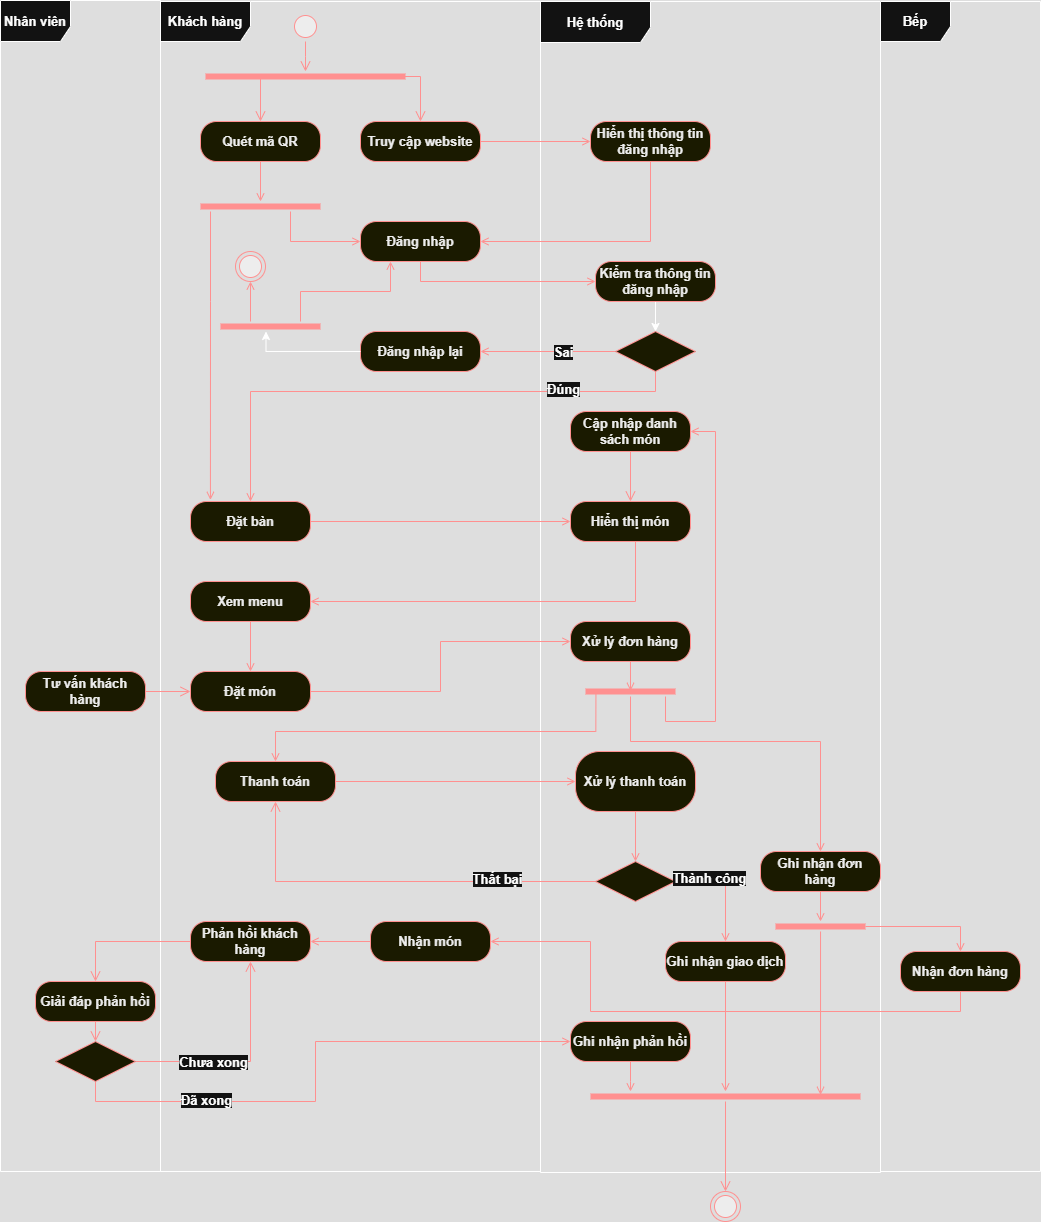
\includegraphics[width=0.9\textwidth]{task21.png}
            \caption{Sơ đồ hoạt động của hệ thống}
            \label{fig:task21}
        \end{figure}
        \subsubsection{Task 2.2 - Sơ đồ trình tự (Sequence diagram)}
        \begin{figure}[H]
            \centering
            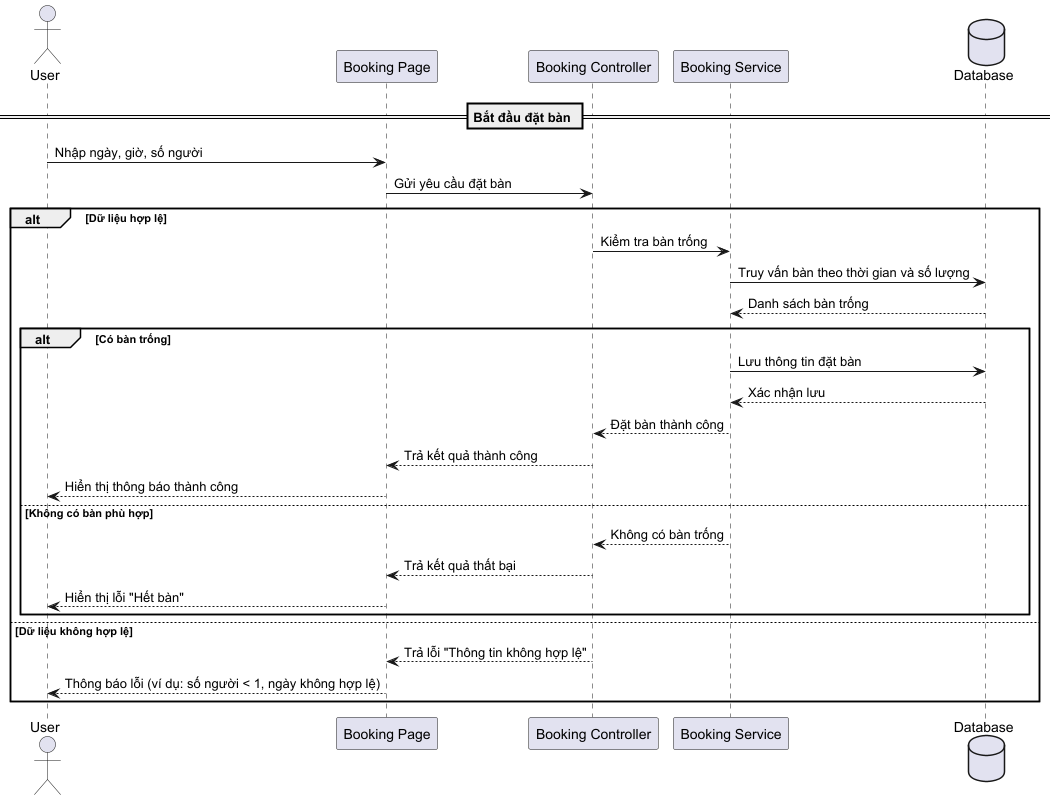
\includegraphics[width=0.9\textwidth]{task22.png}
            \caption{Sơ đồ trình tự của hệ thống}
            \label{fig:task22}
        \end{figure}
        \subsubsection{Task 2.3 - Sơ đồ lớp (Class diagram)}
        \begin{figure}[H]
            \centering
            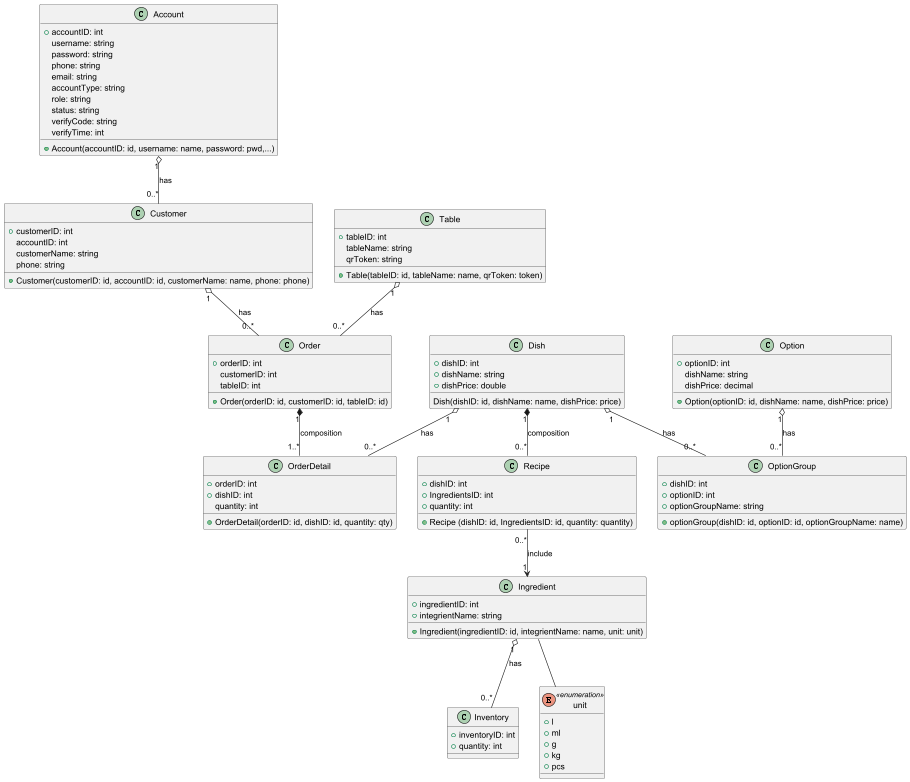
\includegraphics[width=0.9\textwidth]{task23.png}
            \caption{Sơ đồ lớp của hệ thống}
            \label{fig:task23}
        \end{figure}
        \subsubsection{Task 3.2 - Sơ đồ triển khai (Class diagram)}
        \begin{figure}[H]
            \centering
            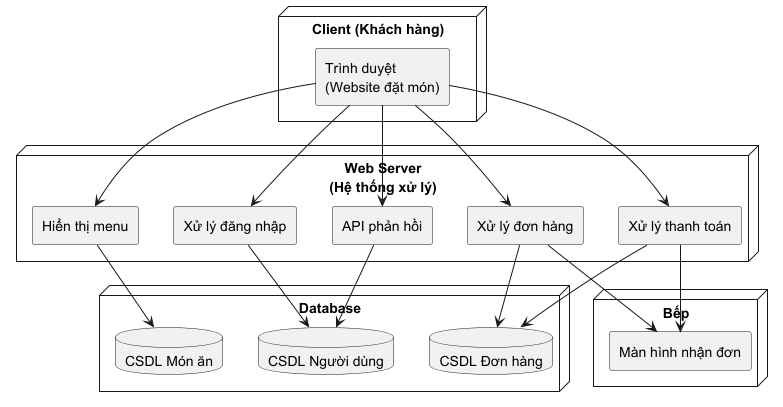
\includegraphics[width=0.9\textwidth]{task32.png}
            \caption{Sơ đồ triển khai của hệ thống}
            \label{fig:task32}
        \end{figure}
    
    \subsection{Các chức năng đã triển khai}
    \begin{itemize}
        \item Quản lý tài khoản và phân quyền người dùng
        \item Quản lý thông tin khách hàng
        \item Quản lý bàn ăn và tạo mã QR
        \item Quản lý đơn hàng và chi tiết đơn hàng
        \item Quản lý thực đơn, món ăn và tùy chọn
        \item Quản lý công thức và nguyên liệu
        \item Quản lý kho hàng
        \item Hỗ trợ thanh toán trực tuyến qua VNPAY
    \end{itemize}


\newpage
%%%%%%%%%%%%%%%%%%%%%%%%%%%%%%%%%
\section{Cấu trúc dự án}
\begin{itemize}
    \item Cấu trúc được dùng trong dự án là một implementation của mẫu thiết kế "Repository Pattern" và kiến trúc MVC (Model-View-Controller) mà NestJS áp dụng. Khi thực thi lệnh nest g resource <tên module> --no-spec trên terminal, NestJS tự động tạo ra một cấu trúc module đầy đủ theo RESTful API.
    \item Luồng thông tin trong cấu trúc này:
Controller: Tiếp nhận HTTP request từ client
DTO (Data Transfer Object): Xác thực và chuyển đổi dữ liệu đầu vào
Service: Xử lý logic nghiệp vụ
Schema: Đại diện cho dữ liệu trong cơ sở dữ liệu
    \item Luồng xử lý: Request → Controller → Service → Schema → Database và ngược lại.
\end{itemize}
\subsection{Tổng quan cấu trúc}

Dự án được tổ chức với cấu trúc thư mục rõ ràng và module hóa:

\begin{verbatim}
Root/
├── .gitignore 
├── README.md                           # Hướng dẫn dự án
├── report.md                           # Báo cáo dự án
│
├── asset/                              # Ảnh và tài liệu
│   ├── diagram/                        # Các diagram UML
│   ├── png/
│
├── backend/                            # Thư mục backend
│   ├── src/                            # Mã nguồn backend
│   │   ├── app.controller.ts           # Controller cấp ứng dụng
│   │   ├── app.module.ts               # Module chính
│   │   ├── app.service.ts              # Service cấp ứng dụng
│   │   ├── main.ts                     # Điểm vào ứng dụng
│   │   ├── auth/                       # Module xác thực người dùng
│   │   ├── decorator/                  # Custom decorators
│   │   ├── mail/                       # Module gửi email
│   │   ├── modules/                    # Các module nghiệp vụ
│   │   └── Util/                       # Tiện ích và helper
│   ├── test/                           # Thư mục test
│   ├── .env.example                    # File mẫu cấu hình môi trường
│   ├── .env                            # Cấu hình môi trường
│   ├── docker-compose.yml              # Cấu hình Docker
│   └── package.json                    # Cấu hình Node.js
│
├── frontend/                           # Thư mục frontend
│   ├── public/                         # Tài nguyên tĩnh
│   ├── src/                            # Mã nguồn frontend
│   │   ├── app/                        # Các trang ứng dụng
│   │   ├── components/                 # Components tái sử dụng
│   │   ├── context/                    # Context và quản lý trạng thái
│   │   └── lib/                        # Thư viện và tiện ích
│   └── package.json                    # Cấu hình Node.js
│
└── report/                             # Báo cáo
    ├── Assignment_report.tex           # File báo cáo
    └── references.bib                  # Tài liệu tham khảo
\end{verbatim}

\subsection{Cấu trúc Backend}

Backend được tổ chức theo kiến trúc module của NestJS, với mỗi đối tượng nghiệp vụ được đóng gói trong một module riêng biệt, bao gồm:

\begin{enumerate}
    \item \textbf{Module}: Quản lý các dependencies và providers
    \item \textbf{Controller}: Xử lý các request HTTP
    \item \textbf{Service}: Xử lý logic nghiệp vụ
    \item \textbf{DTO (Data Transfer Objects)}: Định nghĩa cấu trúc dữ liệu cho input/output
    \item \textbf{Schema}: Định nghĩa cấu trúc dữ liệu MongoDB
\end{enumerate}

\subsection{Cấu trúc Frontend}

Frontend sử dụng Next.js với App Router, tổ chức theo cấu trúc:

\begin{enumerate}
    \item \textbf{app/}: Chứa các trang và routes
    \item \textbf{components/}: Components tái sử dụng
    \item \textbf{context/}: Quản lý trạng thái toàn cục
    \item \textbf{lib/}: Các tiện ích và helper functions
\end{enumerate}

\subsection{Kho lưu trữ trực tuyến}
Dự án được lưu trữ và phát triển trên GitHub tại địa chỉ: \url{https://github.com/Hiennguyen278610/CNPM/commits/main/}. 
Kho lưu trữ này chứa toàn bộ mã nguồn của dự án, bao gồm cả phần frontend và backend, cũng như tài liệu thiết kế và các tài nguyên liên quan.

\newpage

%%%%%%%%%%%%%%%%%%%%%%%%%%%%%%%%%%%%%%%%%%%%%%
\section{Giao diện dự án}
    \subsection{Giao diện được thiết kế}
    
    Giao diện ban đầu của dự án được thiết kế trên nền tảng Figma với liên kết: \url{https://www.figma.com/file/restaurant-ordering-system}
    
    \begin{figure}[H]
        \centering
        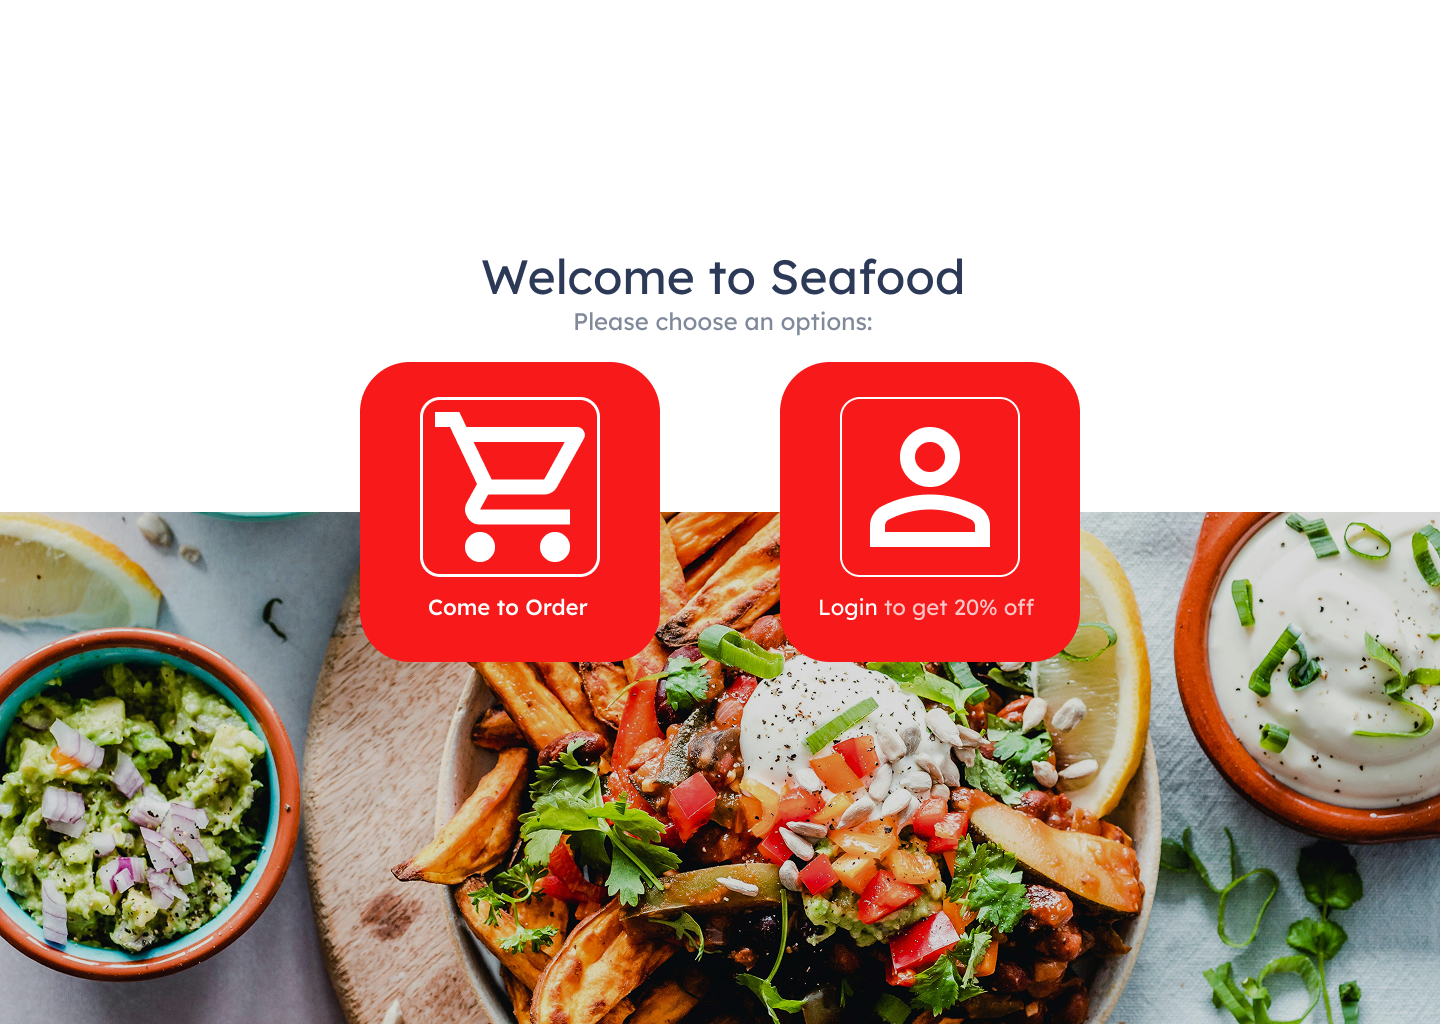
\includegraphics[width=0.8\textwidth]{figmaHome.png}
        \caption{Giao diện trang chủ - Hiển thị thông tin chào mừng và danh mục món ăn phổ biến}
    \end{figure}
    
    \begin{figure}[H]
        \centering
        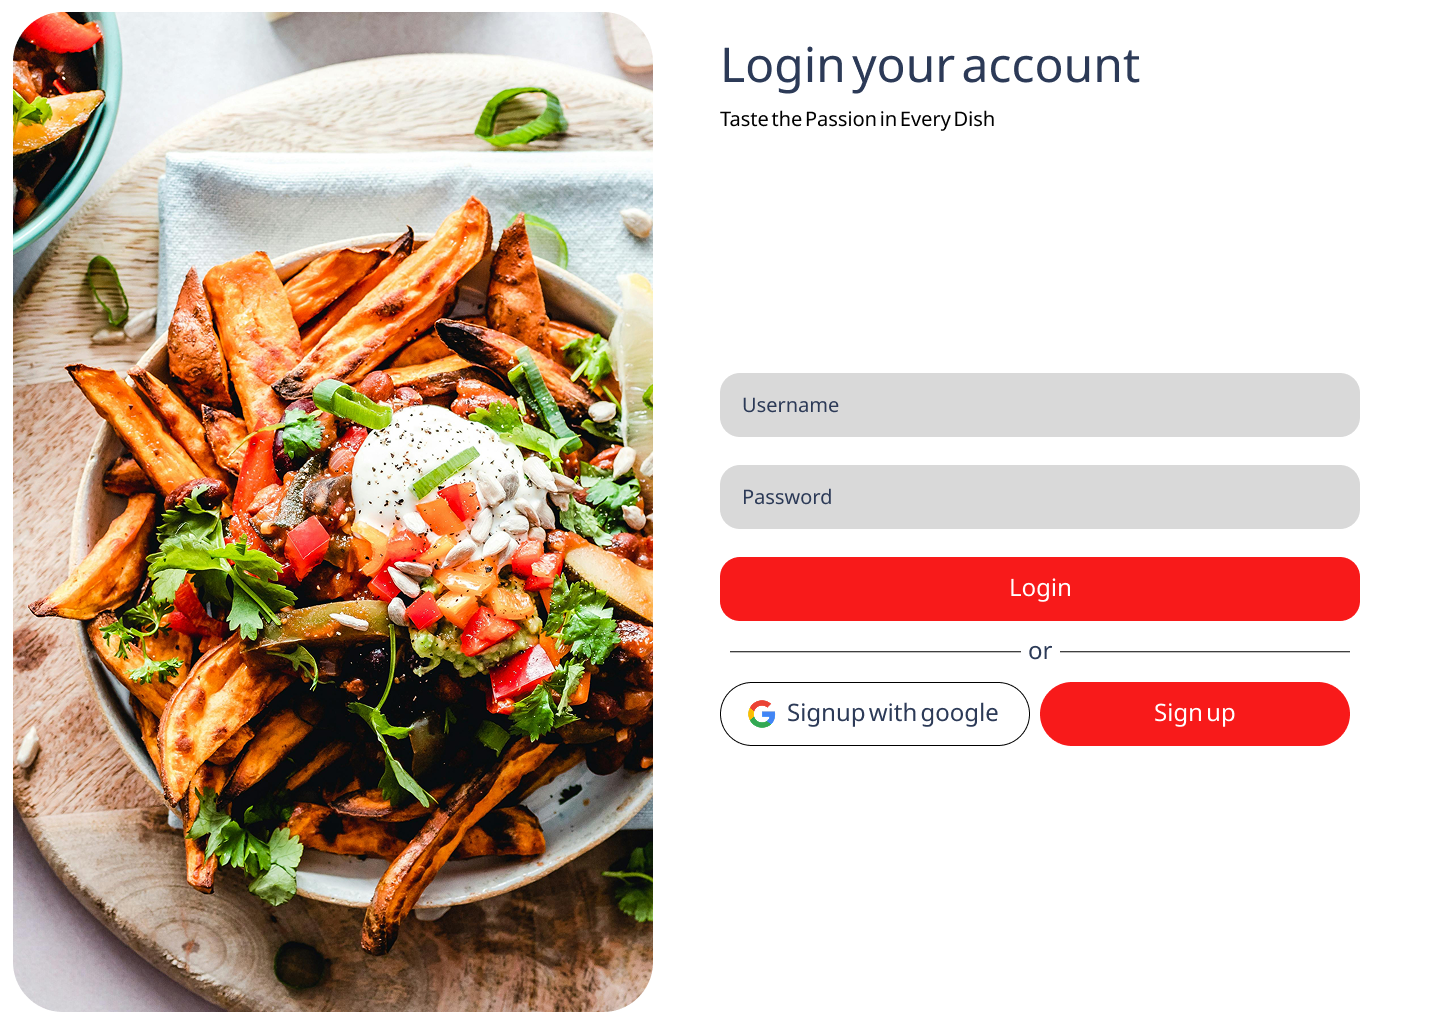
\includegraphics[width=0.8\textwidth]{figmaLogin.png}
        \caption{Giao diện đăng nhập - Cho phép người dùng đăng nhập với email và mật khẩu}
    \end{figure}
    
    \begin{figure}[H]
        \centering
        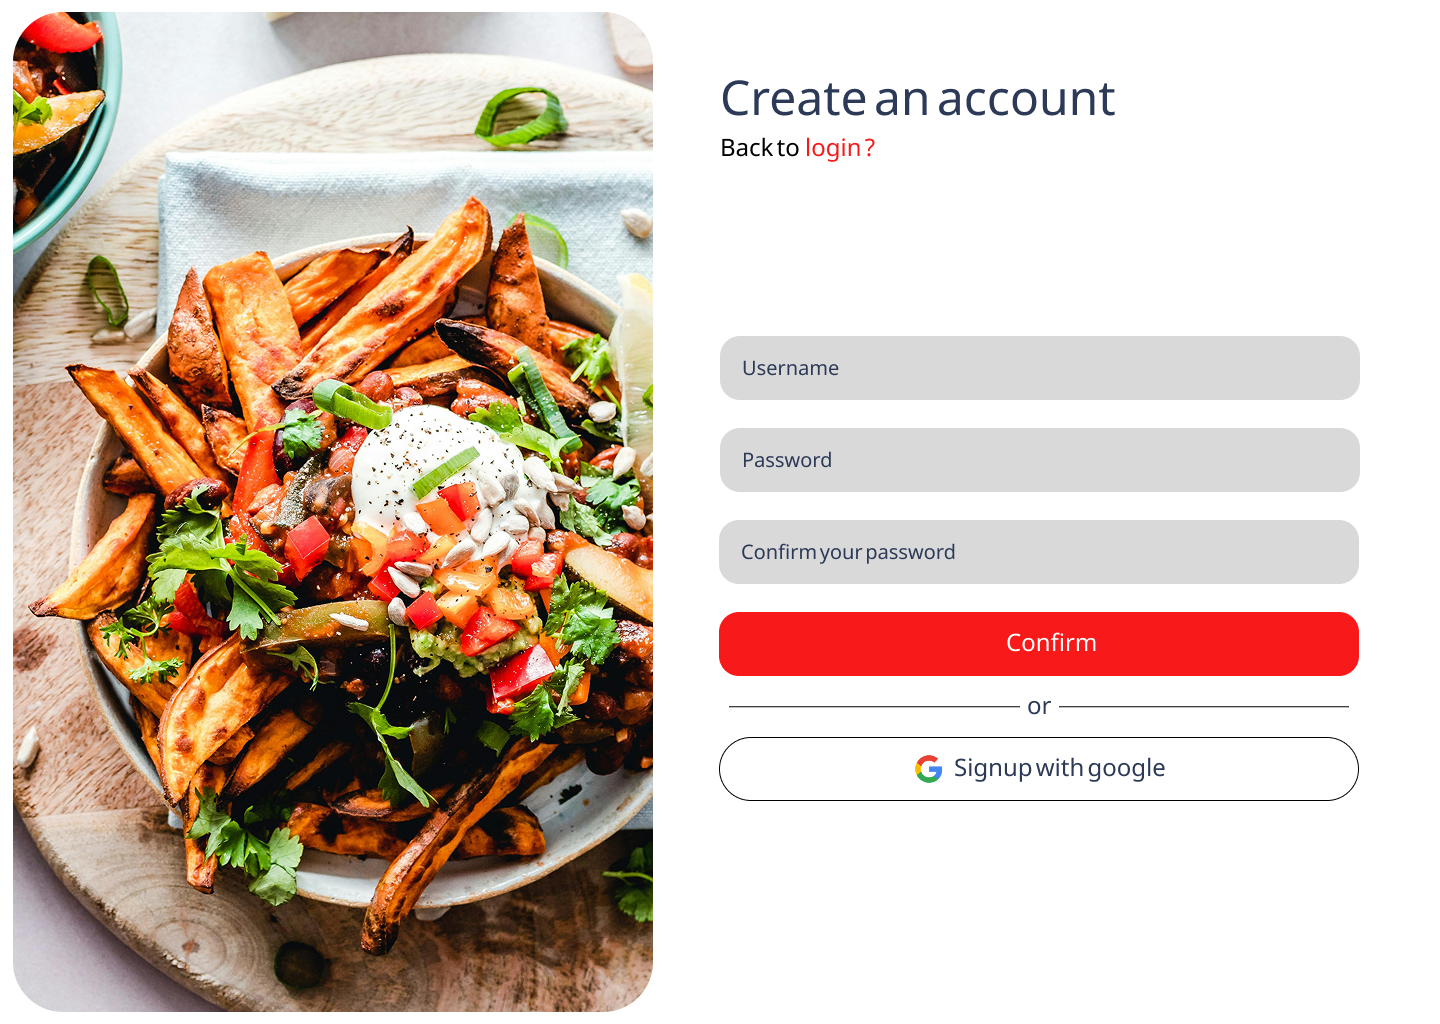
\includegraphics[width=0.8\textwidth]{figmaRegister.png}
        \caption{Giao diện đăng ký - Cho phép người dùng đăng ký tài khoản mới với thông tin cá nhân}
    \end{figure}
    
    \begin{figure}[H]
        \centering
        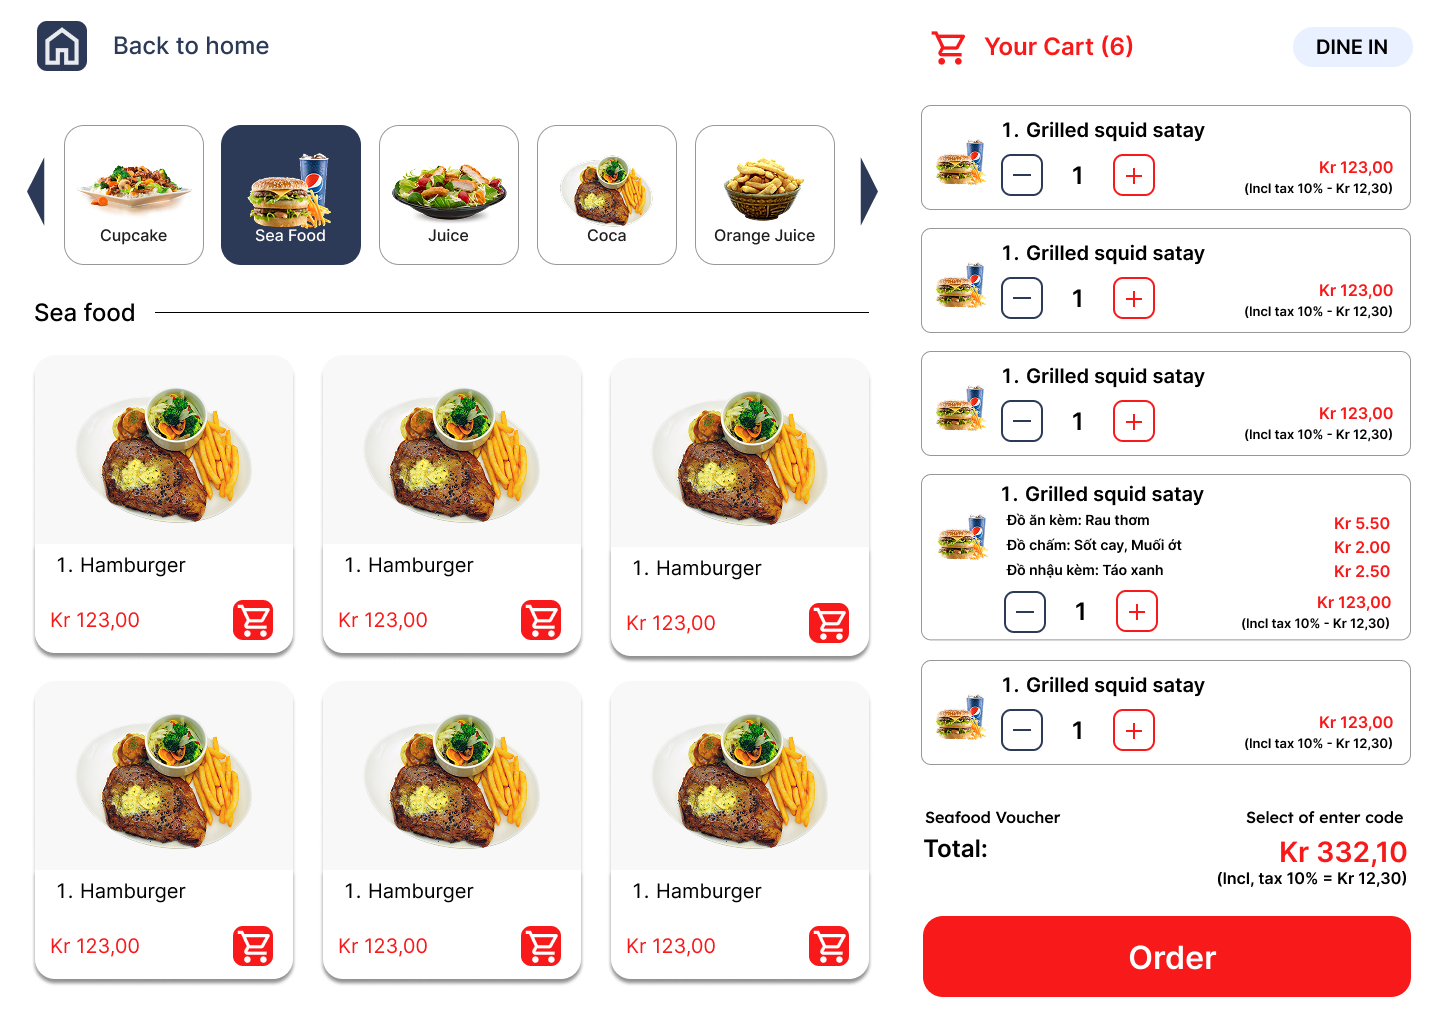
\includegraphics[width=0.8\textwidth]{figmaMenu.png}
        \caption{Giao diện thực đơn - Hiển thị danh sách các món ăn theo từng danh mục}
    \end{figure}
    
    \begin{figure}[H]
        \centering
        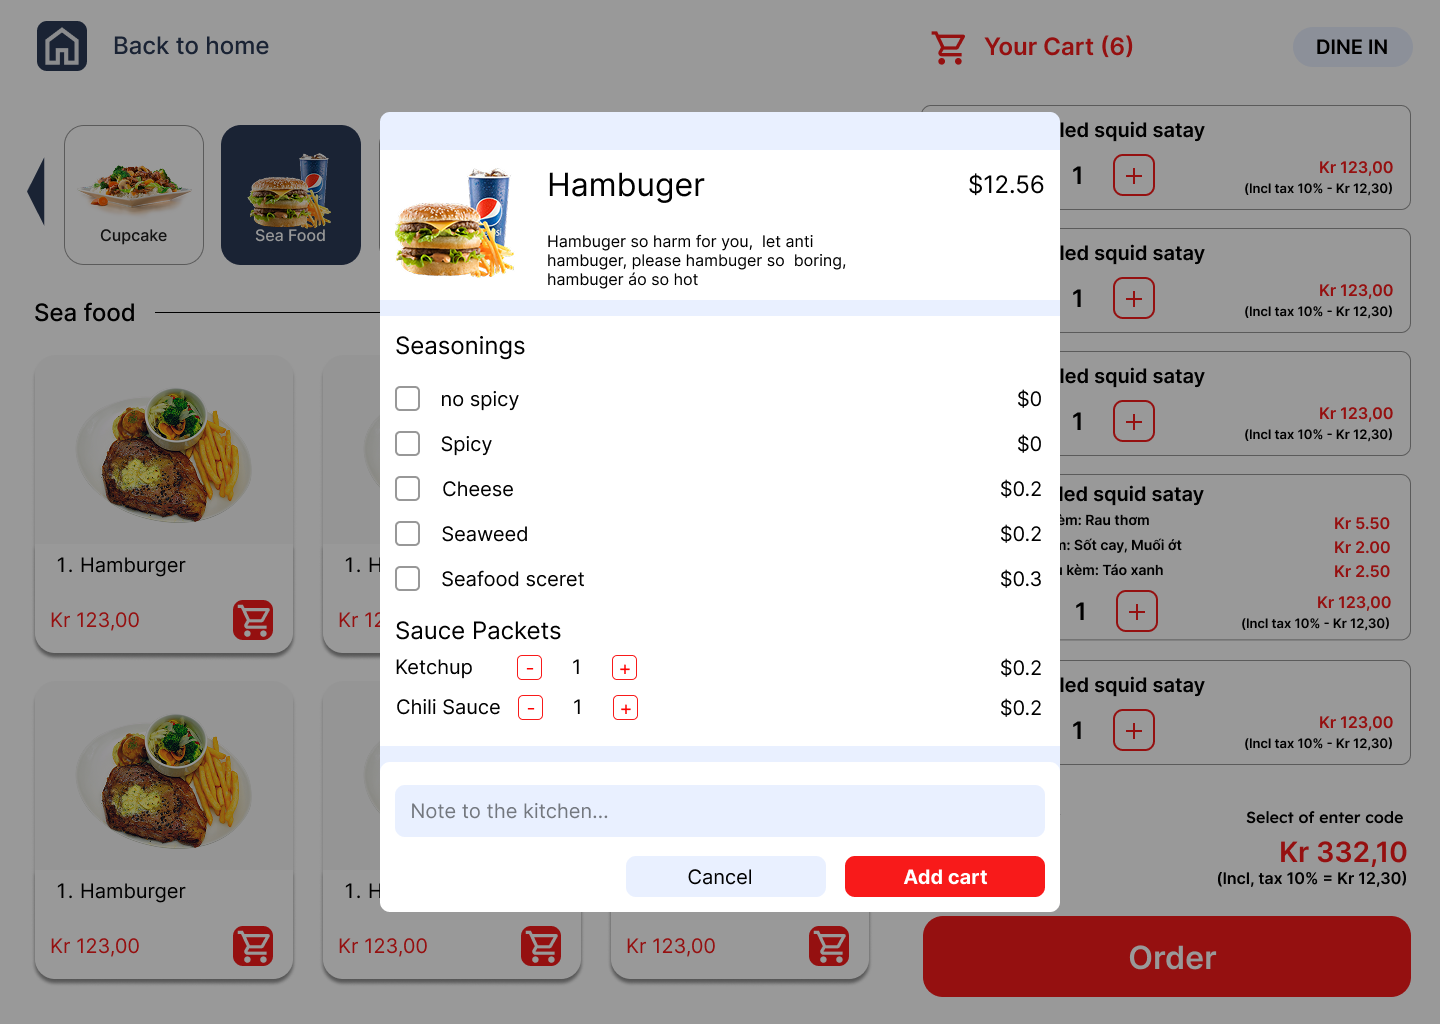
\includegraphics[width=0.8\textwidth]{figmaOrderDetail.png}
        \caption{Giao diện chi tiết đơn hàng - Hiển thị thông tin chi tiết về đơn hàng đã đặt}
    \end{figure}
    
    \begin{figure}[H]
        \centering
        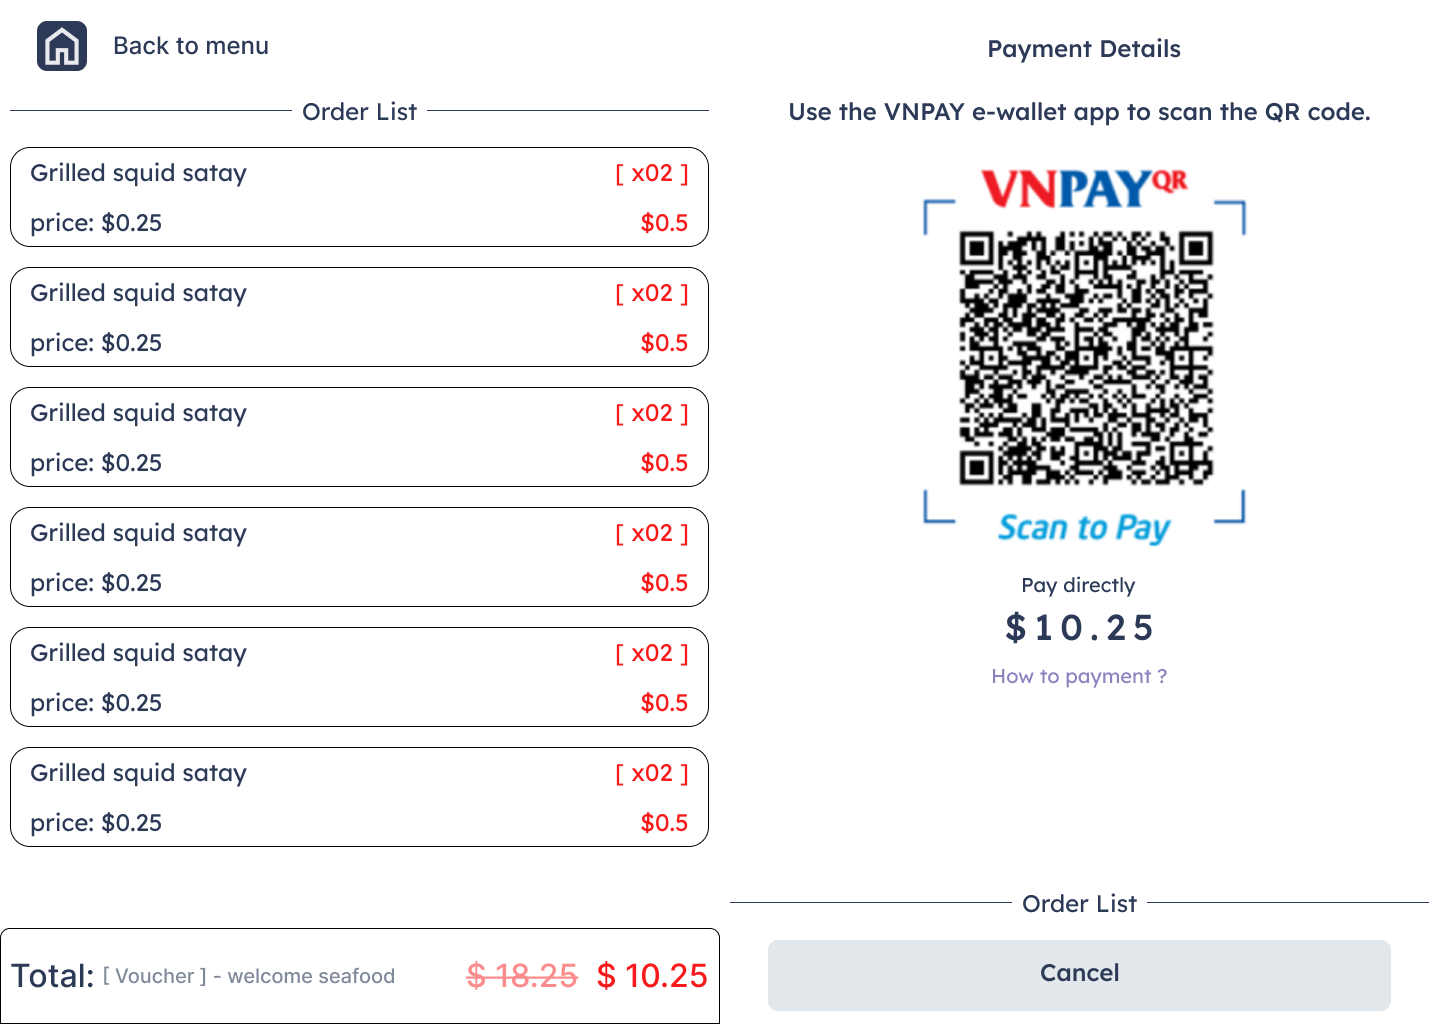
\includegraphics[width=0.8\textwidth]{figmaPayment.png}
        \caption{Giao diện thanh toán - Cho phép người dùng lựa chọn phương thức thanh toán và hoàn tất đơn hàng}
    \end{figure}
    
    \subsection{Giao diện được triển khai}
    \begin{figure}[H]
        \centering
        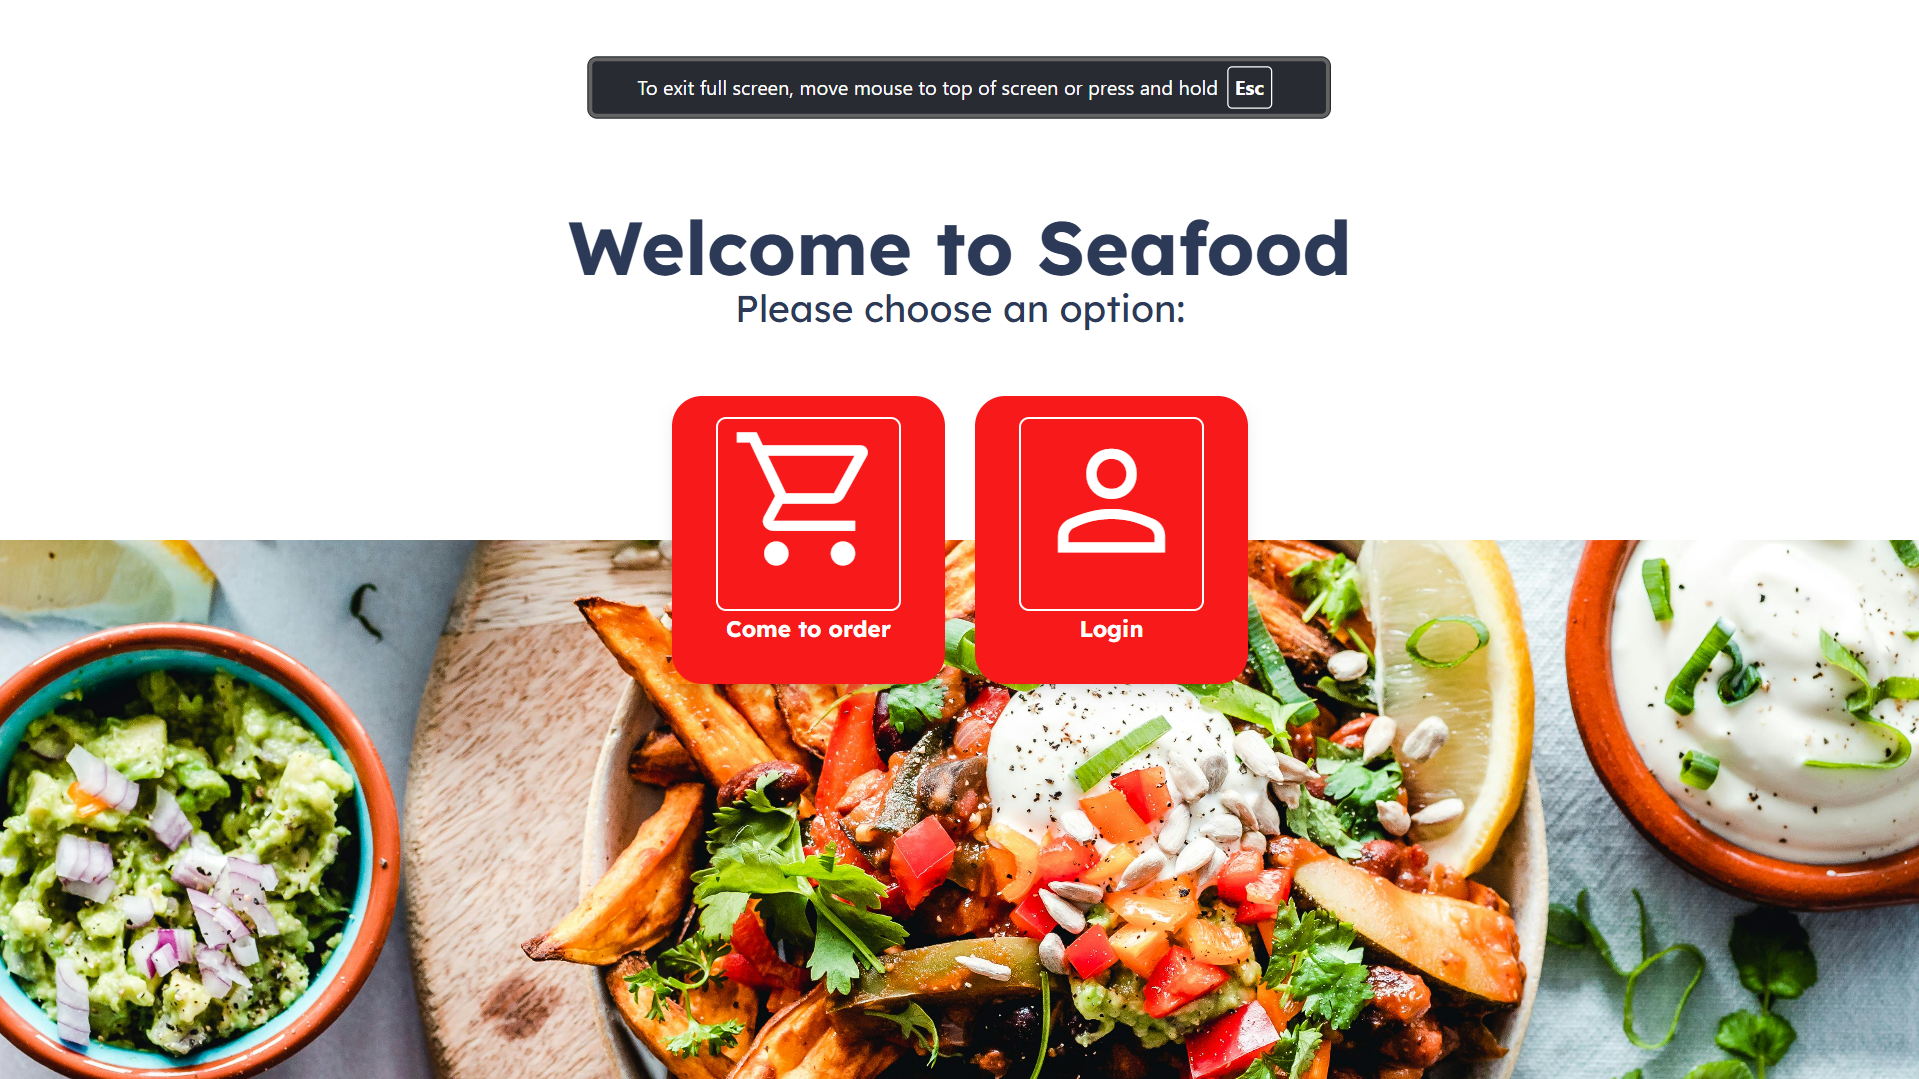
\includegraphics[width=0.8\textwidth]{home.png}
        \caption{Giao diện trang chủ - Hiển thị thông tin chào mừng và danh mục món ăn phổ biến}
    \end{figure}
    
    \begin{figure}[H]
        \centering
        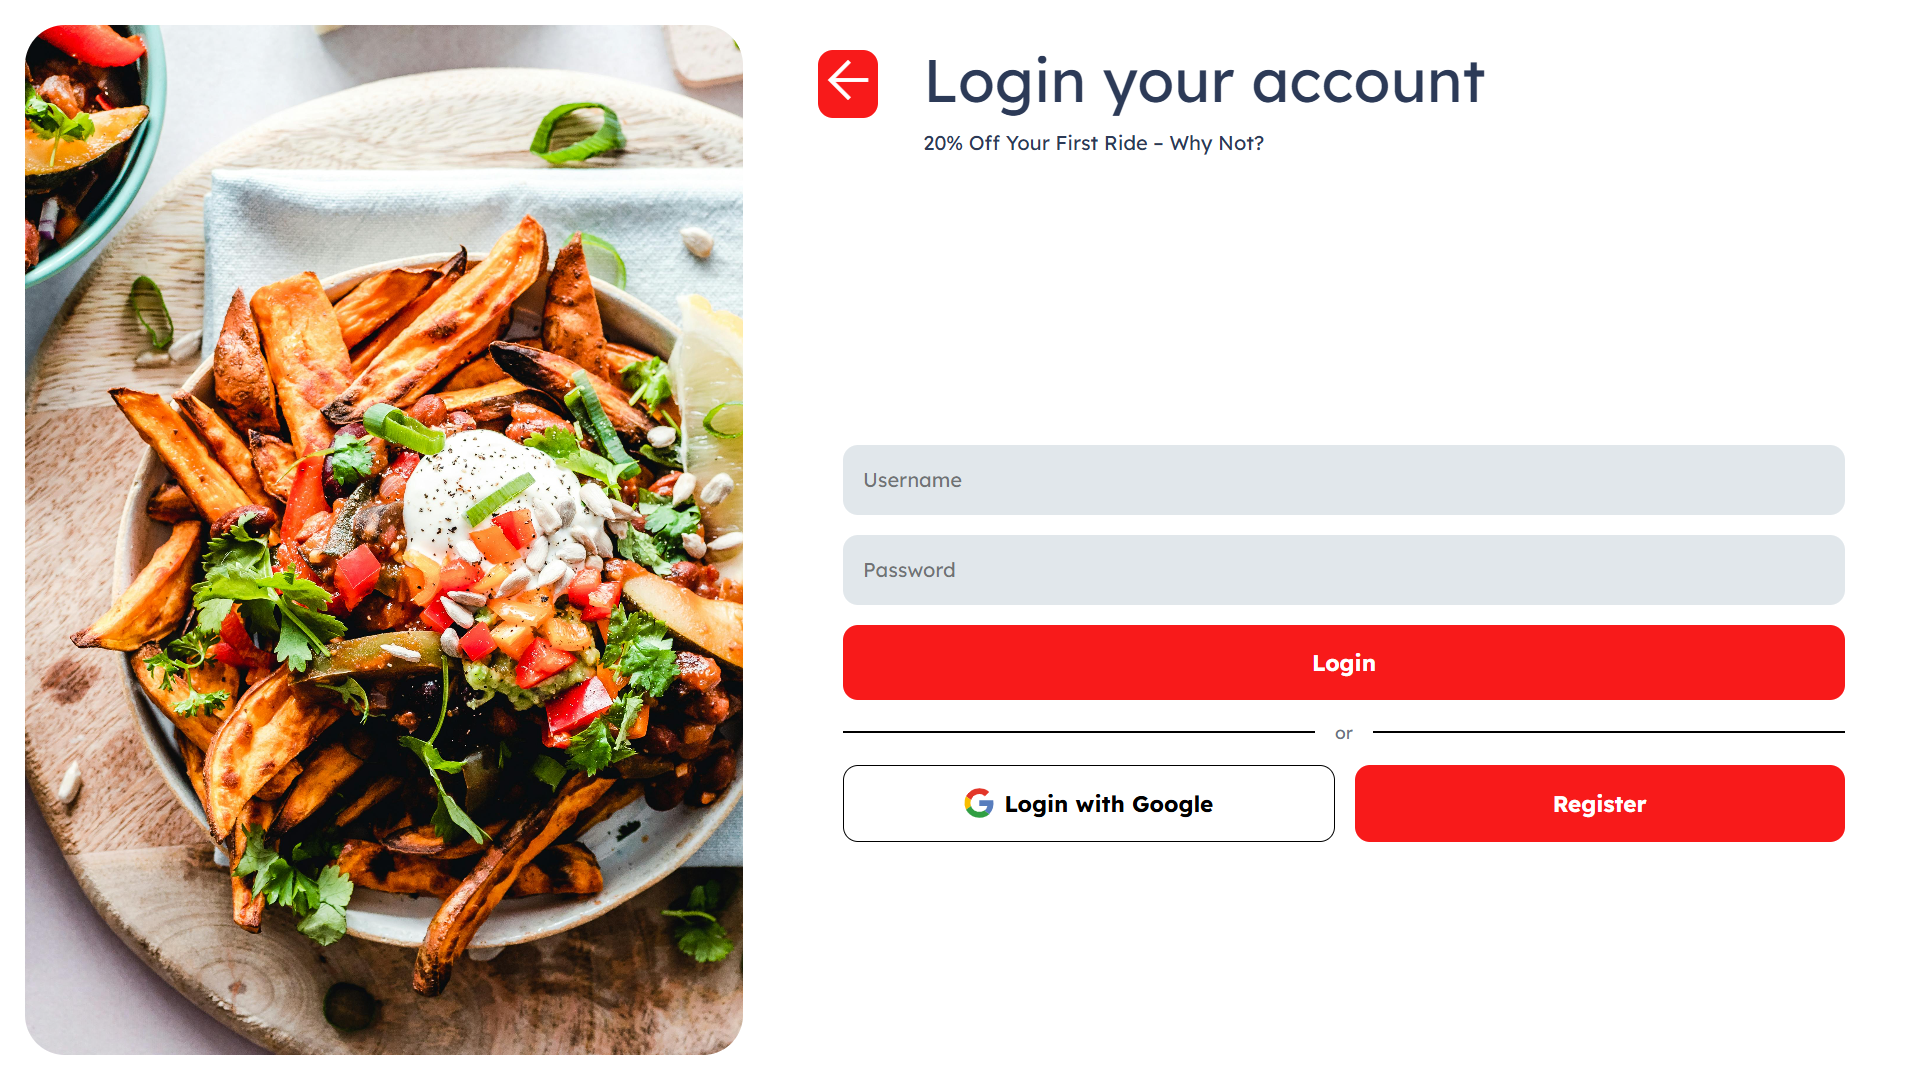
\includegraphics[width=0.8\textwidth]{login.png}
        \caption{Giao diện đăng nhập - Cho phép người dùng đăng nhập với email và mật khẩu}
    \end{figure}
    
    \begin{figure}[H]
        \centering
        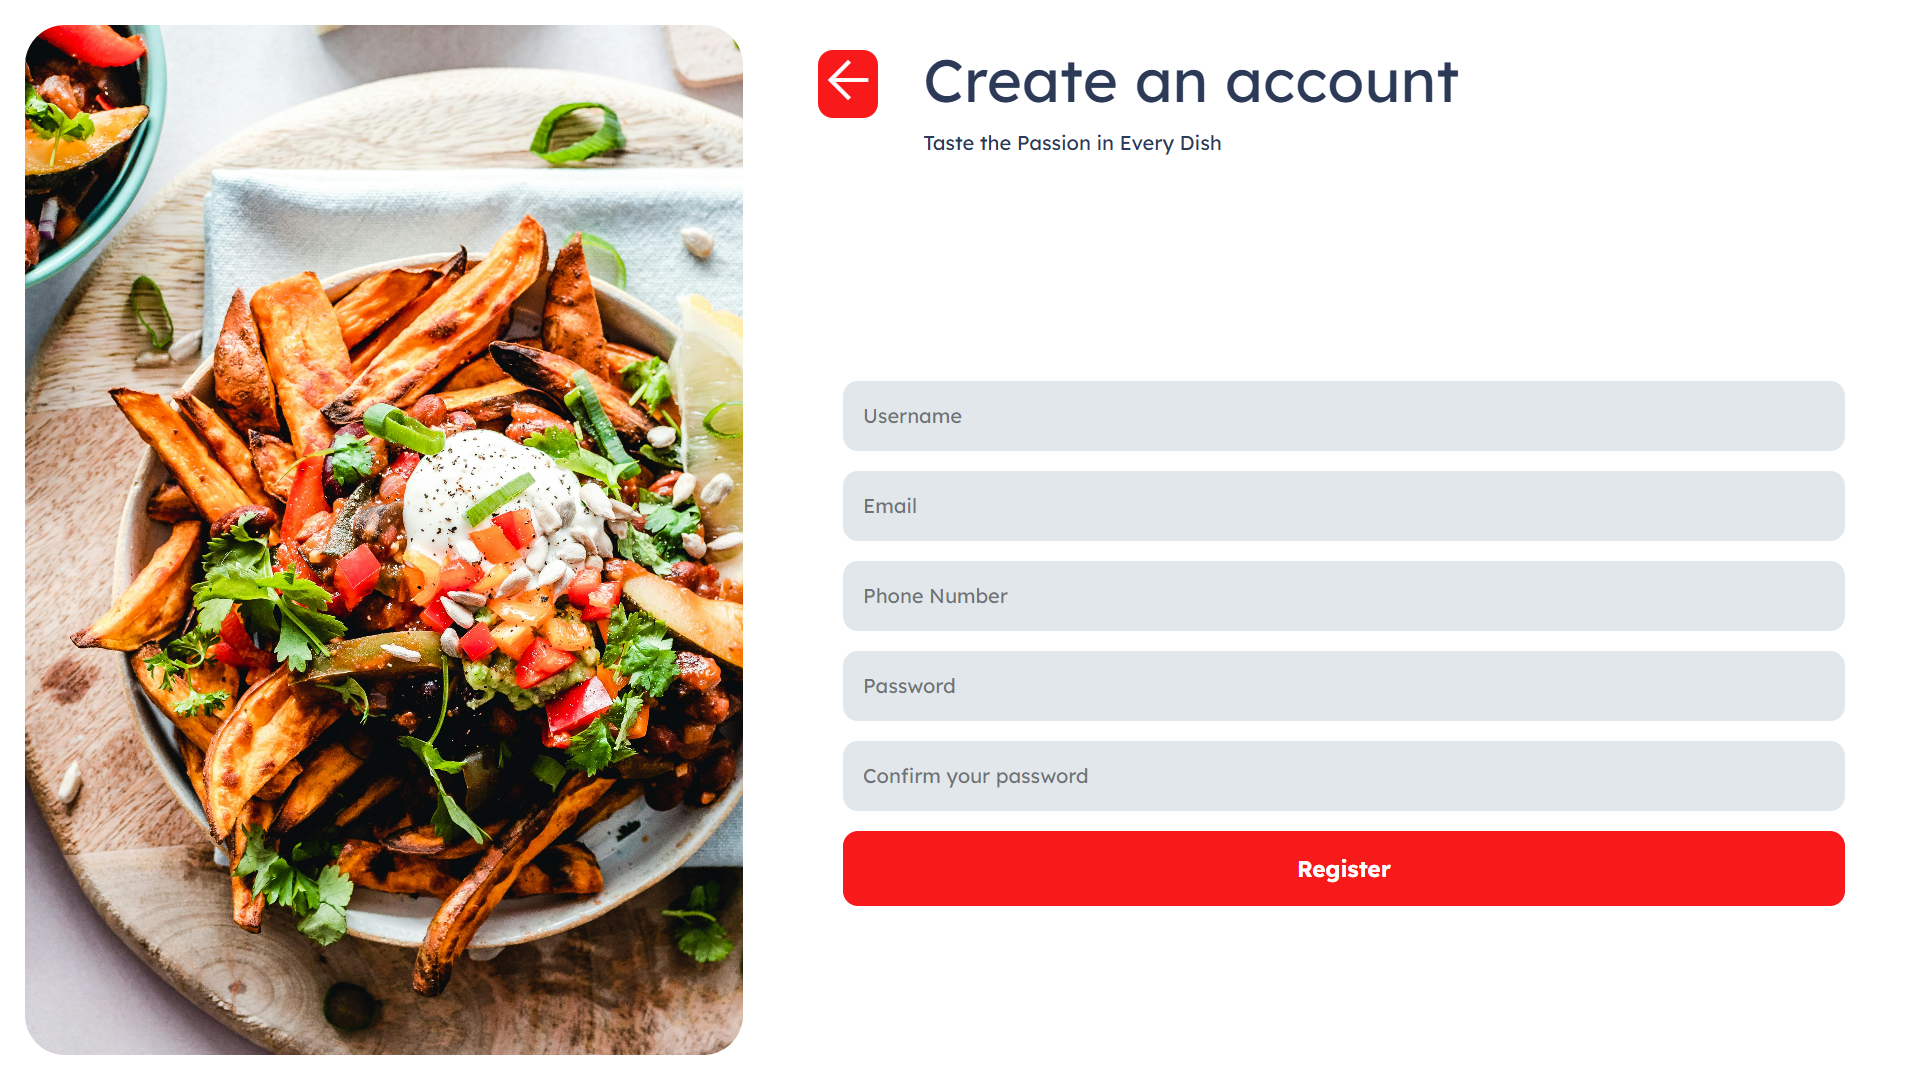
\includegraphics[width=0.8\textwidth]{register.png}
        \caption{Giao diện đăng ký - Cho phép người dùng đăng ký tài khoản mới với thông tin cá nhân}
    \end{figure}
    
    \begin{figure}[H]
        \centering
        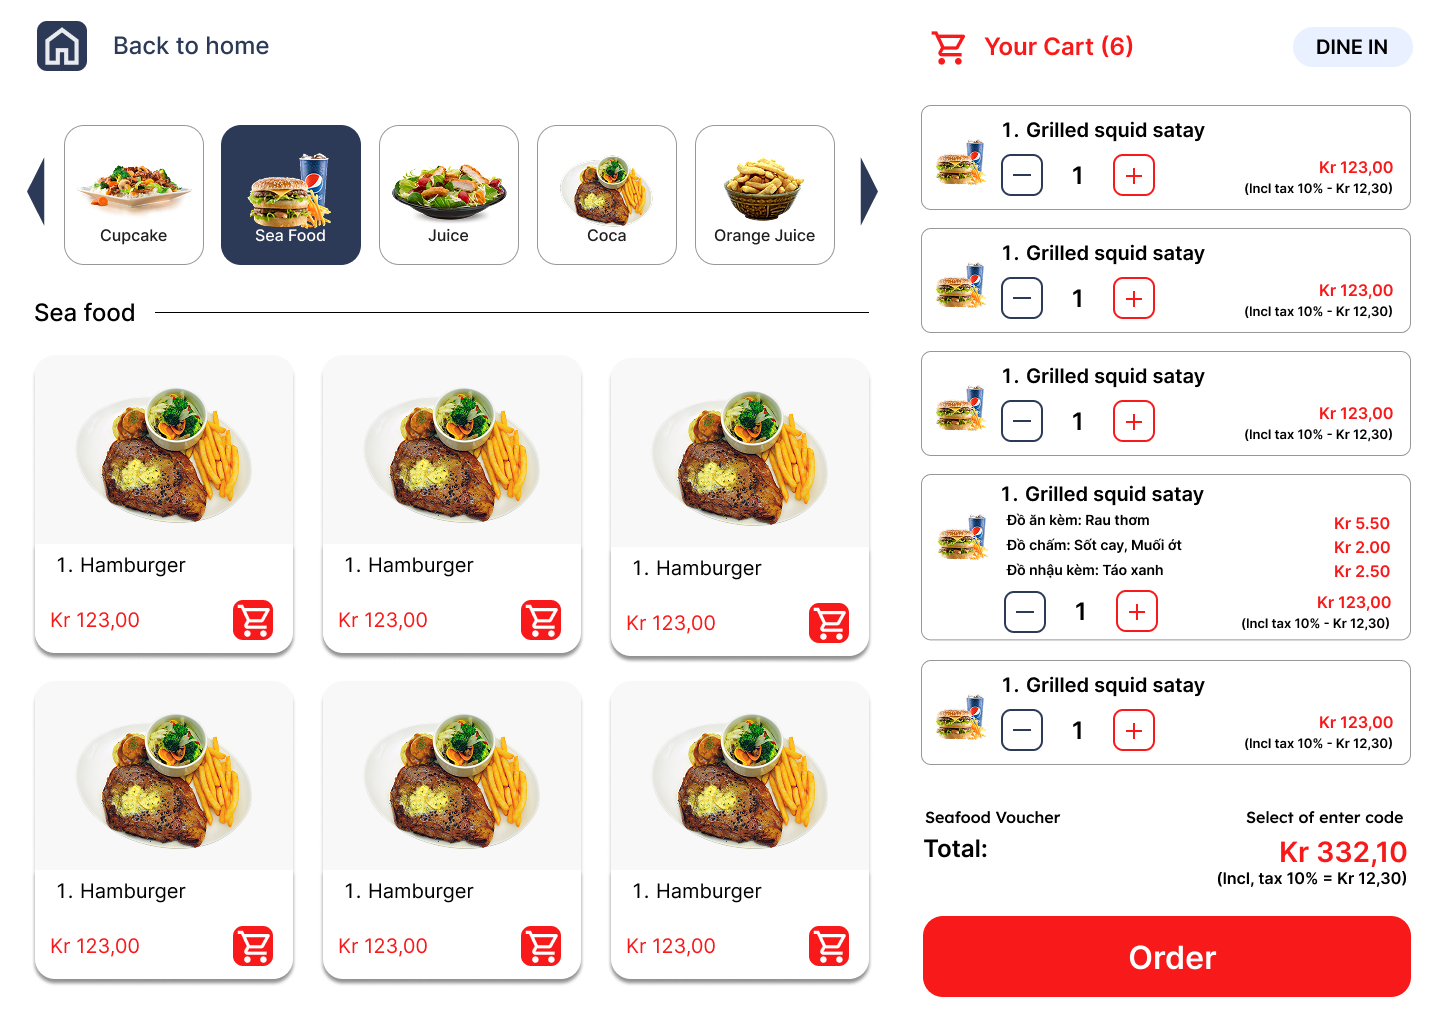
\includegraphics[width=0.8\textwidth]{figmaMenu.png}
        \caption{Giao diện thực đơn - Hiển thị danh sách các món ăn theo từng danh mục}
    \end{figure}
    
    \begin{figure}[H]
        \centering
        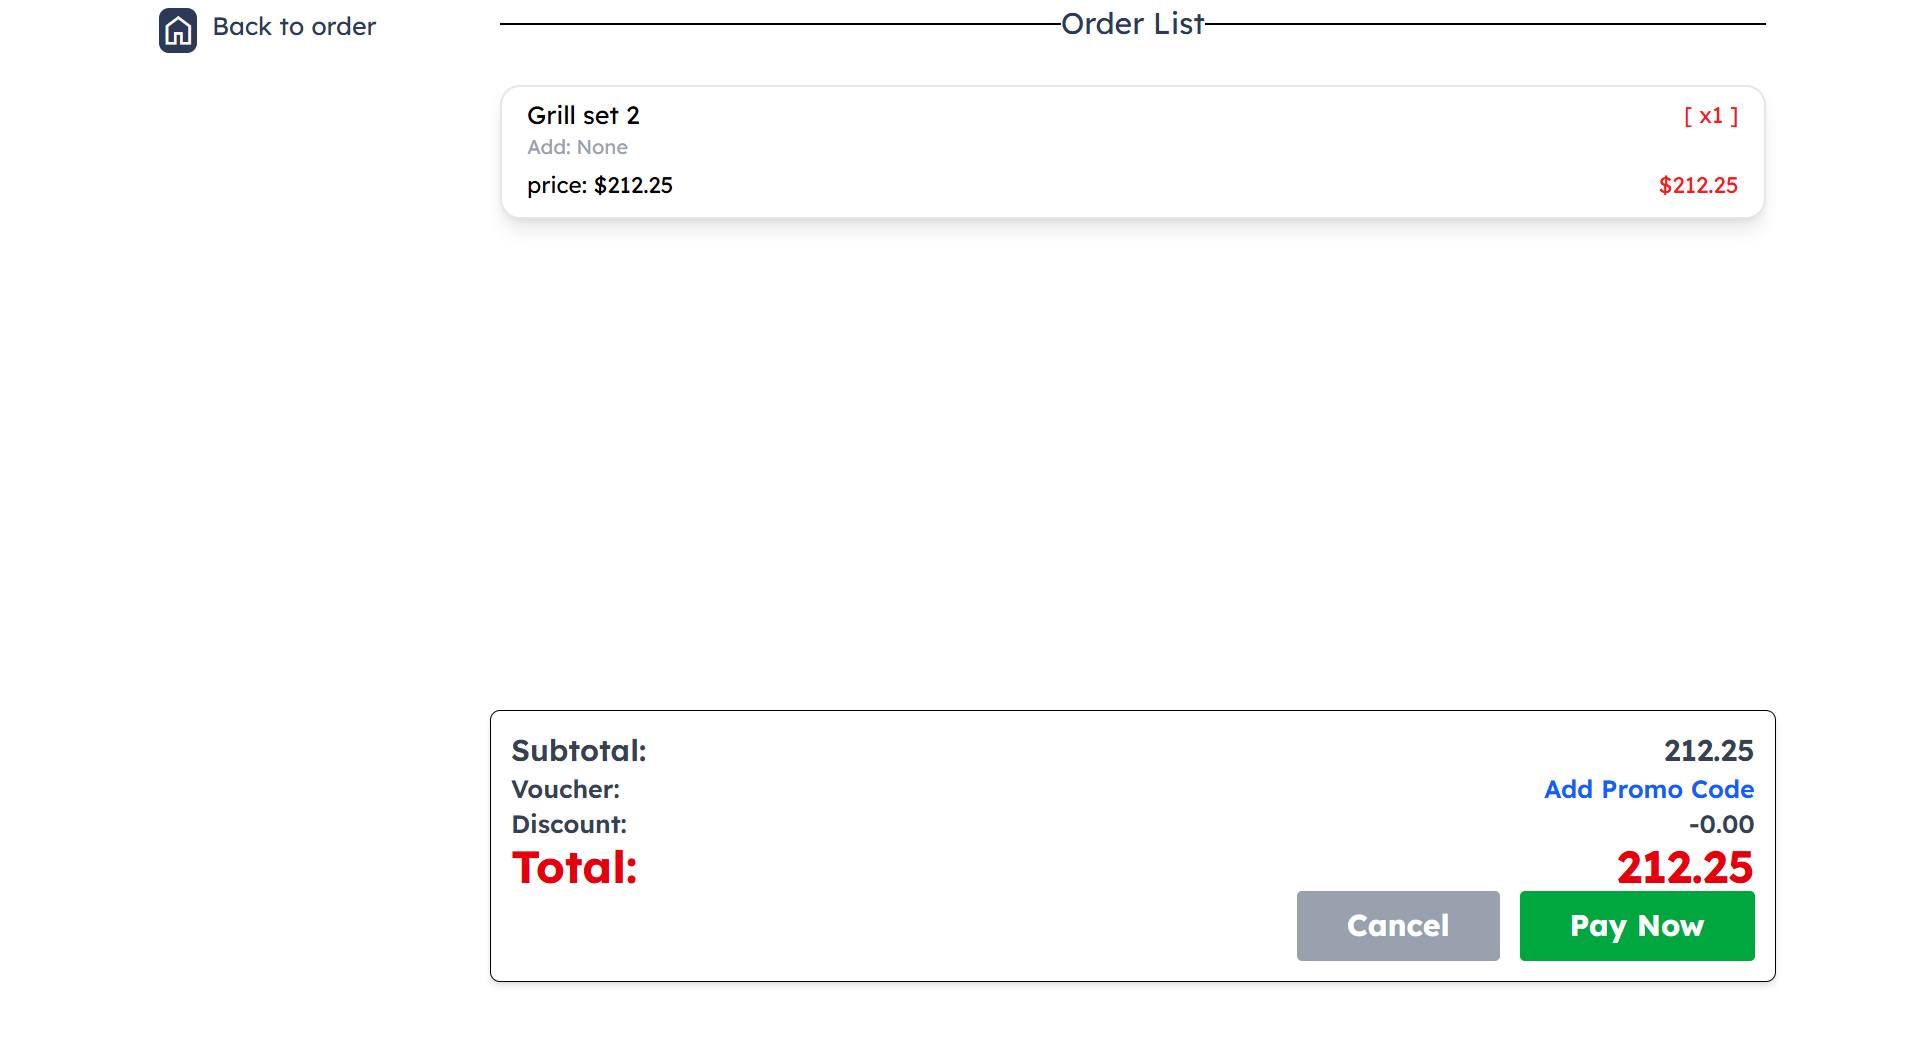
\includegraphics[width=0.8\textwidth]{payment.png}
        \caption{Giao diện thanh toán - Cho phép người dùng lựa chọn phương thức thanh toán và hoàn tất đơn hàng}
    \end{figure}

\newpage

%%%%%%%%%%%%%%%%%%%%%%%%%%%%%%%%%
 \section{Triển khai dự án}
    \subsection{Hướng dẫn cài đặt và triển khai}
        \subsubsection{Yêu cầu hệ thống}
        \begin{itemize}
             \item Node.js phiên bản mới nhất
            \item Docker và Docker Compose
            \item Windows Subsystem for Linux (WSL2)
            \item Git
        \end{itemize}
        
        \subsubsection{Các bước cài đặt}
        \begin{enumerate}
            \item Clone repository:
            \begin{verbatim}
                git clone <repository-url>
                cd cnpmProject
            \end{verbatim}
            
            \item Cài đặt dependencies Frontend:
            \begin{verbatim}
                cd frontend
                npm install
                npm run dev
            \end{verbatim}
            
            \item Cài đặt dependencies Backend:
            \begin{verbatim}
                cd ../backend
                npm install
                npm run dev
            \end{verbatim}
            
            \item Cấu hình Docker cho MongoDB:
            \begin{verbatim}
                cd backend
                docker compose -p restaurant-mongodb up -d
            \end{verbatim}
        \end{enumerate}

    \subsection{Tính năng và luồng hoạt động}
        \subsubsection{Xác thực và phân quyền}
        \begin{itemize}
            \item Đăng ký và xác thực tài khoản qua email
            \item Đăng nhập với JWT authentication
        \end{itemize}
        
        \subsubsection{Quản lý đơn hàng}
        \begin{itemize}
            \item Khách hàng quét mã QR của bàn để đặt món
            \item Hệ thống tạo đơn hàng và chi tiết đơn hàng
            \item Nhân viên nhận và xử lý đơn hàng
            \item Kiểm tra tình trạng đơn hàng real-time
        \end{itemize}
        
        \subsubsection{Quản lý thực đơn}
        \begin{itemize}
            \item Thêm, sửa, xóa món ăn và tùy chọn
            \item Quản lý công thức và nguyên liệu
            \item Cập nhật trạng thái món (còn/hết)
        \end{itemize}
        
        \subsubsection{Thanh toán}
        \begin{itemize}
            \item Thanh toán trực tiếp tại nhà hàng
            \item Thanh toán trực tuyến qua VNPAY
        \end{itemize}

    \subsection{Kỹ thuật triển khai}
        \subsubsection{Validation và Error Handling}
        \begin{itemize}
            \item Sử dụng ValidationPipe trong NestJS để kiểm tra dữ liệu đầu vào
            \item Xử lý lỗi với HTTP exceptions
            \item Bảo mật với bcrypt cho mật khẩu
        \end{itemize}
        
        \subsubsection{Kết nối cơ sở dữ liệu}
        \begin{itemize}
            \item Sử dụng Mongoose để kết nối với MongoDB
            \item Thiết lập schemas với định nghĩa kiểu dữ liệu TypeScript
            \item Quản lý quan hệ giữa các collections
        \end{itemize}
   

%%%%%%%%%%%%%%%%%%%%%%%%%%%%%%%%%
\section{Kết luận và hướng phát triển}
    \subsection{Kết luận}
    Hệ thống quản lý nhà hàng đã được triển khai thành công với kiến trúc hiện đại, đáp ứng được các yêu cầu nghiệp vụ cơ bản. Việc sử dụng các công nghệ như Next.js, NestJS và MongoDB đã mang lại hiệu suất cao và trải nghiệm người dùng tốt.
    
    Dự án đã hoàn thành tất cả các Task từ 1-5, bao gồm:
    \begin{itemize}
        \item Khai thác yêu cầu và xác định phạm vi dự án
        \item Mô hình hóa hệ thống với các sơ đồ UML
        \item Thiết kế kiến trúc phù hợp cho hệ thống
        \item Triển khai MVP cho các màn hình menu và chi tiết món ăn
        \item Triển khai các tính năng chính của hệ thống
    \end{itemize}
    
    \subsection{Hướng phát triển tương lai}
    Các hướng phát triển tiếp theo cho dự án bao gồm:
    \begin{itemize}
        \item Tích hợp phân tích dữ liệu và báo cáo thống kê
        \item Tích hợp công cụ quản lý nhà hàng đầy đủ và nâng cao
        \item Phát triển ứng dụng di động đồng bộ với web
        \item Tích hợp thêm các cổng thanh toán khác
        \item Hệ thống đánh giá và phản hồi từ khách hàng
        \item Tự động hóa quy trình kiểm tra và cảnh báo tồn kho
    \end{itemize}

\newpage

\begin{thebibliography}{80}

\bibitem{YT}
``\textbf{Restaurant Management System Guide}'',
\textit{Youtube Video Reference}, 
\textbf{link: https://www.youtube.com/watch?v=5Ul\_rUuoUZE},
lần truy cập cuối: 01/05/2024.

\bibitem{NEXT}
Next.js Documentation,
``\textbf{link: https://nextjs.org/docs}'',
\textit{The React Framework for the Web},
lần truy cập cuối: 03/05/2024.

\bibitem{NEST}
NestJS Documentation,
``\textbf{link: https://docs.nestjs.com/}'',
\textit{A progressive Node.js framework},
lần truy cập cuối: 03/05/2024.

\bibitem{MONGO}
MongoDB Documentation,
``\textbf{link: https://www.mongodb.com/docs/}'',
\textit{MongoDB Documentation},
lần truy cập cuối: 03/05/2024.

\bibitem{DOCKER}
Docker Documentation,
``\textbf{link: https://docs.docker.com/}'',
\textit{Docker Documentation},
lần truy cập cuối: 03/05/2024.

\bibitem{REACTJS}
React Documentation,
``\textbf{link: https://react.dev/reference/react}'',
\textit{A JavaScript library for building user interfaces},
lần truy cập cuối: 05/05/2024.

\bibitem{TAILWIND}
Tailwind CSS Documentation,
``\textbf{link: https://tailwindcss.com/docs}'',
\textit{A utility-first CSS framework},
lần truy cập cuối: 05/05/2024.

\bibitem{NPM}
npm Documentation,
``\textbf{link: https://docs.npmjs.com/}'',
\textit{The world's largest software registry},
lần truy cập cuối: 05/05/2024.

\bibitem{SWIPER}
Swiper Documentation,
``\textbf{link: https://swiperjs.com/get-started}'',
\textit{The Most Modern Mobile Touch Slider},
lần truy cập cuối: 05/05/2024.


\end{thebibliography}
\end{document}

